\documentclass{article}

\usepackage{tikz}
\usetikzlibrary{positioning}

\begin{document}

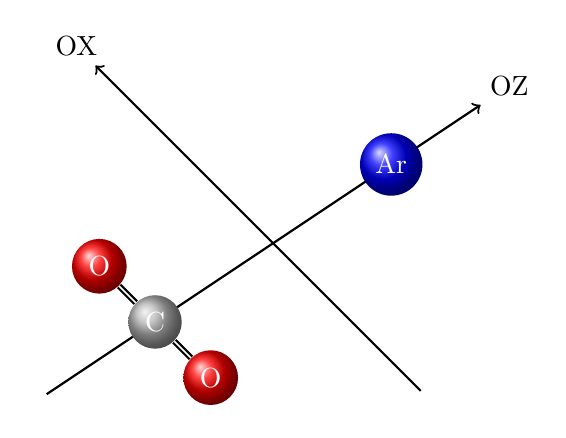
\begin{tikzpicture}
	[oxygen/.style={ball color = red, circle, text = white}, 
	carbon/.style={ball color = black!30, circle, text = white},
	argon/.style={ball color = blue, circle, text = white}]
	\node (z1) at (4.5, 3) {OZ};
	\node (z2) at (-1.5, -1) {}
		edge [->, thick] (z1);

	\node (x1) at (-1, 3.5) {OX};
	\node (x3) at (3.5, -1) {}
		edge [->, thick] (x1); 

	\node (carbon) [carbon] {C};
	\node (oxygen1) [oxygen, below right of = carbon] {O}
		edge [double, thick] (carbon);
	\node (oxygen2) [oxygen, above left of = carbon] {O}
		edge [double, thick] (carbon);
	\node[argon] (argon) at (3, 2) {Ar};
\end{tikzpicture}


\end{document}
